%!TEX root=kdd15_workshop_main.tex
\section{Introduction}
\subsection{Graph Partitioning}
Distributed algorithms that operate on sparse data, such as large-scale graph mining, nearly always encounter load-balance and network communication as their bottleneck. Graph partitioning is the problem of dividing a graph into separate components with particular properties. In parallel computing the objective is generally equally-sized partitions (to favor load balance) and the minimization of inter-partition edges (to minimize communication).

Formally, we wish to partition the nodes of a graph into $k$ balanced components with capacity $(1+\epsilon)\frac{N}{k}$, such that the number of edges that cross partition boundaries is minimized. Partitioning with these two requirements can be reduced to the minimum-bisection problem~\cite{Garey:1979:CIG:578533} and is therefore NP-Complete. For this reason it is computationally infeasible to expect an optimal solution for even modest-sized graphs, and approximation techniques are common.

% scenario
An effective partitioning of a graph can greatly improve the performance of graph algorithms. Consider a parallel Breadth-First Search (BFS) where a graph's vertices (vertex edge lists) are partitioned between two machines.
During each BFS step, each process must communicate all newly explored vertices to the owner of those vertices.
In Figure~\ref{fig:0}, if we have 4 processes, all 14 nonzeros in the non-diagonal blocks must be communicated at some point.
A good partitioner concentrates nonzeros in the diagonal blocks, thereby reducing communication (which is the main bottleneck in almost all graph computations).

Offline graph partitioning algorithms have existed for decades.
They work by storing the graph in memory with complete information about the edges.
Hundreds of variants of these algorithms exist and range from spatial methods~\cite{Gilbert95geometricmesh} to spectral methods~\cite{arora2009expander}.
Some of the most effective offline graph partitioners are multi-level partitioners, which recursively contract the graph to a small number of vertices, and then heuristically optimize the partitioning while expanding back to the original graph~\cite{karypis1998multilevel}.

\paragraph{Why Use Streaming Partitioning?}
The most salient property of streaming partitioning is its speed: it can partition the graph in a single sweep, with $O(|E|)$ memory access, storage, and run time. Existing graph partitioners require the whole graph to be represented in memory, whereas streaming graph partitioning can process vertices as they arrive.

For example, partitioning a 26GB Twitter graph can take nearly a day using the fastest offline algorithms, but can take a matter of minutes using a streaming algorithm, with similar partition quality~\cite{tsourakakis2012fennel}.
This also suggests that we could do multiple passes of a streaming partitioner (using the same or different heuristics) to further improve the partitioning, all in a fraction of the time that an offline partitioner would take to terminate.


\begin{figure}[h]
\centering
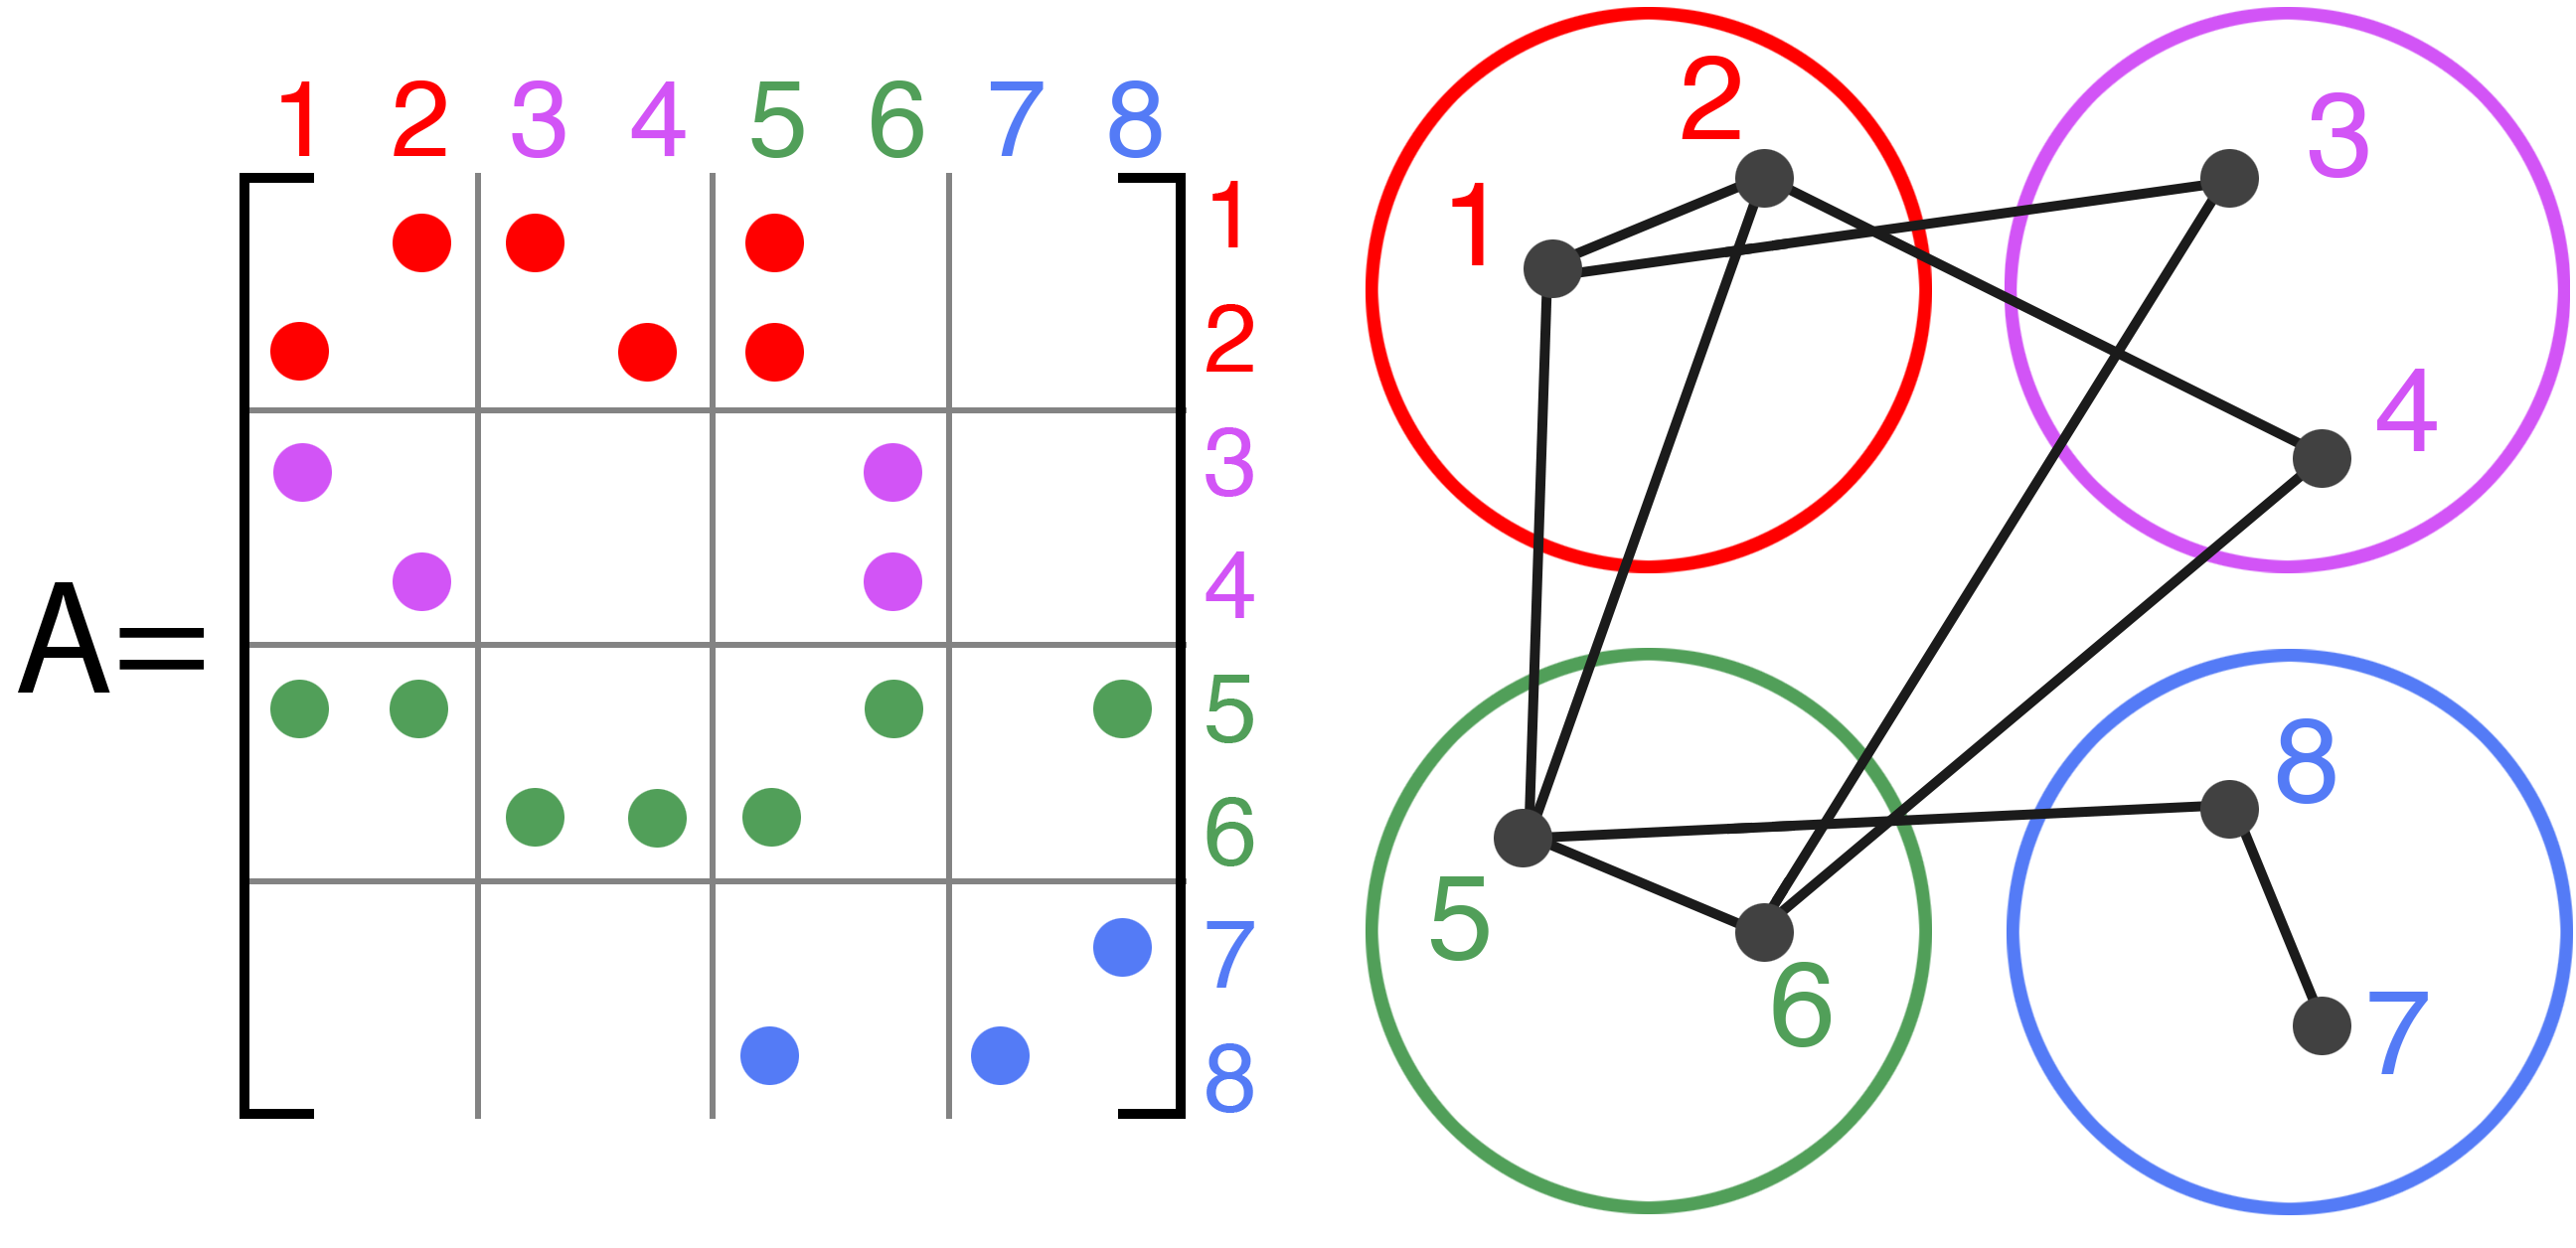
\includegraphics[width=0.85\columnwidth] {figures/graphpart1.png}
\caption[Caption for]{Graph 4-partition shown with corresponding adjacency matrix}
\label{fig:0}
\end{figure}


Streaming graph partitioning has gained traction in the last few years~\cite{DBLP:journals/corr/abs-1212-1121,Stanton:2012:SGP:2339530.2339722,tsourakakis2012fennel}.
As graphs grow to the point where they do not fit into memory or must be distributed to compute nodes on the fly, we need new methods that support partitioning on only limited information.
In the streaming model, input data (vertices) arrive sequentially from a generating source (such as a web-crawler), and must be partitioned as they arrive.

Streaming partitioning is dependent on the order in which vertices arrive.
A web crawler might generate vertices in an order that represents a Breadth-First or Depth-First traversal of the web, or we may even receive vertices in a random order.
An analysis of streaming algorithms may also consider an adversarial ordering that produces the worst possible results~\cite{Stanton:2012:SGP:2339530.2339722}.

We have created \ourmethod, a fast, iterative, distributed streaming graph partitioner.
It works by restreaming the graph with tempered partition parameters to achieve a fast, parallel \textit{k}-partitioning.
We make the following contributions:
\begin{itemize}
\item A \textbf{scalable} distributed partitioner implementation using MPI.
\item Support for \textbf{streaming} partitioning regardless of stream order.
\item An \textbf{iterative} approach that creates quality partitions.
\end{itemize}



